\section{Proposed approach}\label{seq:model}
%\todo{the subsubsections here are going to be merged}
In this section we first define the proposed approach and explain the objectives used to train the model.
%
The details of the training process are presented in \autoref{seq:training}.

\subsection{Bag of Attribute}
\begin{figure}[t]
\begin{subfigure}{.57\textwidth}\centering
    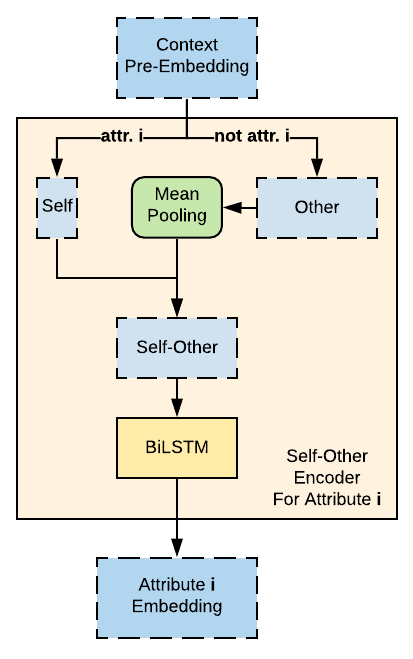
\includegraphics[height=6cm, keepaspectratio]{img/boa_self_other_encoder.png}  
    \caption{Self-other attribute encoder for an attribute \textit{i}.}\label{fig:self-other}
\end{subfigure}
\begin{subfigure}{.42\textwidth}\centering
    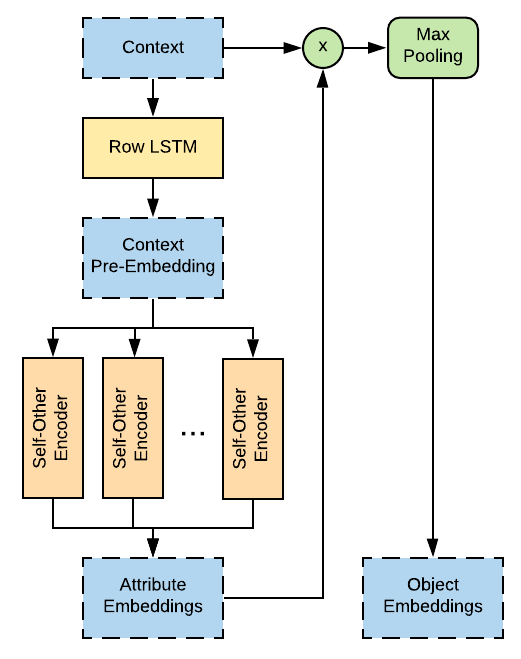
\includegraphics[height=6cm, keepaspectratio]{img/boa_encoder.png}  
    \caption{BoA encoder architecture.}\label{fig:encoder}
\end{subfigure}
\caption{Schematic representation of the BoA architecture. Blue blocks correspond to tensors, orange to neural components and green blocks to non-neural computations. Arrows joining represent concatenation of tensors.} \label{fig:model}
\end{figure}

The proposed model take a formal context as input, and produces embeddings for its attributes.
Then, object embeddings are computed using the embeddings of the attributes and the formal context.
We call our model \textit{Bag of Attribute} (BoA), by reference to \textit{Bag of Word} (BoW), because it considers attributes as an unordered set to produce the object and attribute embeddings.
It has three main components: a pre-embedding generator, an attribute encoder called \textit{self-other encoder} to compute the attribute embedding, and an object encoder. 
The structure of the model is schematized in \autoref{fig:model}.
%
As BoA is trained as a VAE on formal contexts, we also have a decoder.
%
Its input is the concatenation of an attribute embedding and an object embedding.
The decoder itself is a MLP predicting if the object has the attribute ($1$) or not ($0$).
A sigmoid function applied on the output ensures it is in $[0,1]$.
%
For the variational aspect of the model, a $\mu$ and $\sigma$ vector is produced for each attribute.
The sampling of the attribute embeddings is done before the generation of object embeddings.



%\subsubsection{Self-Other Attribute Encoder}
In FCA, the order of the attributes in the dataset do not matter for the final result: if an attribute $a$ appears in \nth{3} or \nth{20}, it won't affect in which concepts' intents it appears.
To capture this property, the attribute encoder processes each attribute in a similar manner:
each attribute is compared to all the other attributes, for each object of the dataset. 
%
In practice, the column of the attribute (called \emph{self}) is compared to an unordered composition of all the other attributes (called \emph{other}).
This \emph{other} summary is the average-pooling of those attributes.
\emph{Self} and \emph{other} are then processed by a bi-LSTM, with the object dimension as the sequence dimension.
The last hidden state of the bi-LSTM is processed with a feed-forward layer into an embedding that represent the attribute.
The structure of the attribute encoder is presented on \autoref{fig:self-other}.

%\subsubsection{Pre-Embedding}
Using unordered composition directly on the binary formal context is problematic: for example, it will prevent the model from differentiating when an attribute $a_1$ is present and $a_2$ is not from when $a_2$ is present and not $a_1$.
The same kind of problem arises with standard embedding methods using a learned vector to represent each possible value: in our example, if we replace in $C$ every $1$ with the same embedding $emb_1$ and every $0$ by $emb_0$, the model is still unable to determine if $emb_0$ stands for $a_1$ or $a_2$.
%The main reason is that the order is not taken into account.
To avoid this issue, we need an embedding model that produces slightly different embeddings for each attribute with the same input. An LSTM typically fit this requirement, as it won't produce the same output for the same input at different time-steps.
For this reason, we apply a LSTM on each row of $C$ before the \textit{self-other encoder}.

%\subsubsection{Object Embedding}
Finally, the object embeddings are computed from the context and the attribute embeddings.
An unordered composition function, the element-wise maximum, is applied to all the attributes present for an object to create its embedding.

%\subsubsection{Time Complexity}
From the structure of the model, we compute the asymptotic time complexity of embedding a formal context as $\theta(|O| \times |A|^2)$. In comparison, applying a linear embedding (the most basic embedding) to each cell has a complexity of $\theta(|O| \times |A|)$, and LSTM embedding models applied to the cells (like our pre-embedding) have a similar complexity.


\subsection{Training Objective}
We train our BoA model using the four objectives.
%
The first two are the KL divergence and the reconstruction loss.
In our case we predict between two classes ($1$ and $0$), so we use the \textit{binary cross entropy} loss for reconstruction.
As the sampling happens before the computation of the object embeddings, the KL divergence is applied on the attribute embeddings exclusively.
%
On top of that we use metric learning with the new \textit{co-intent similarity} (see \autoref{def:co-intent}), and the number of concept.
We use the \textit{mean square error} (MSE) as the loss function.

We use MLPs to predict the co-intent similarity and number of concepts.
For co-intent similarity the input is the concatenated embeddings of two attributes.
We add a sigmoid output function to make sure the predicted similarity is in $[0,1]$.
%
We apply a max-pooling over the attribute embeddings before predicting the number of concepts.
This setting corresponds to a \textit{deep averaging network} (DAN)~\cite{dan:2015:iyyer}.

Predicting the number of concepts from the context, without actually computing the intents, helps when generating the concepts using neural models.
Indeed, knowing how many elements to generate beforehand facilitates the generation process. \todo{Alain: As a remark, counting the number of concepts of a context is \#P-complete (and so, is a "hard" task to achieve)}

We need both ``equal'' and ``different'' attributes to use metric learning on attribute embeddings.
Nonetheless, even if we consider equivalent attributes ($\{a_1\}' = \{a_2\}'$) as ``equal'', they are usually rare within a given context.
For the metric learning process, we use our co-intent similarity to compare attributes. That way we avoid the issues of ``equal'' and ``different'' attributes.
Co-intent similarity ranges from $0$, for attributes never appearing in the same intents, to $1$, for attributes always appearing together or for identical attributes.

\begin{definition}\label{def:co-intent}
For two given attributes from the same context, we call \emph{pairwise co-intent similarity} the ratio of intents containing both attributes over the intents containing either of the attributes.
In cases where no intent contain the attributes (both attributes are empty or padding columns), the similarity is set to $1$.
\autoref{equ:co-intent} is the exact formula of the co-intent similarity.
\end{definition}
\begin{equation}
\text{co-intent}(a_1, a_2) = 
%
\left\{
    \begin{array}{l}
        1 \text{~~~ if } |\{i\in I; a_1 \in i\}| + |\{i\in I; a_2 \in i\}| = 0 \\\\
        \dfrac{2 \times |\{i\in I; a_1 \in i, a_2 \in i\}|}{|\{i\in I; a_1 \in i\}| + |\{i\in I; a_2 \in i\}|} \text{ otherwise.}
    \end{array}
\right.
\label{equ:co-intent}
\end{equation}

%\subsubsection:
% It corresponds to the rate off co-appearance of two attributes within the intents.
% More precisely, it is the ratio of intents containing both attributes over the intents containing either of the attributes.





